% ============================================================
% WORK_ELEVEN: Filtro adaptativo LMS
% ============================================================

\subsection{WORK\_ELEVEN: Filtro adaptativo LMS}

Se implementó el algoritmo LMS (Ec.~\ref{eq:lms}) completamente desde
cero en \texttt{lms\_lab/lms.py}, actualizando el vector de pesos
muestra a muestra según la regla de actualización, sin recurrir a
ninguna función de filtrado adaptativo ya construida por una librería
externa. Esta decisión de diseño es deliberada: el objetivo del
laboratorio es verificar experimentalmente, con código propio y
auditable, que el comportamiento teórico de LMS efectivamente se
manifiesta en la práctica, y no simplemente invocar una caja negra que
produzca resultados correctos sin evidenciar el mecanismo interno.

\subsubsection{Identificación de sistema}

El primer experimento aborda el problema clásico de identificación
ciega de sistemas: se define un filtro FIR desconocido de 5
coeficientes (\texttt{unknown\_system.py}), se lo excita con una señal
de entrada conocida (ruido blanco), y se registra únicamente el par
entrada/salida resultante —exactamente la información disponible en un
escenario real donde el sistema interno es inaccesible y solo se puede
observar su comportamiento externo. LMS utiliza esa entrada como
$x[n]$ y la salida del sistema desconocido como la señal deseada
$d[n]$, y ajusta sus propios 5 pesos tratando de reproducir la
relación entrada-salida observada.

Los resultados (Fig.~\ref{fig:work_eleven_t1_w},
\ref{fig:work_eleven_t1_e}) muestran que los cinco pesos adaptados
convergen de forma monótona y sin oscilación visible hacia los cinco
coeficientes reales del sistema desconocido, alcanzando un error de
identificación $\lVert w_{\text{estimado}} - w_{\text{real}} \rVert = 0$
dentro de la precisión numérica de \texttt{float64}. Este resultado es
significativo porque confirma que LMS no solo minimiza el error de
predicción observable (la diferencia entre $d[n]$ y $y[n]$), sino que
efectivamente recupera los parámetros internos reales del sistema —una
propiedad que no está garantizada en general para cualquier algoritmo
de minimización de error, pero que sí se cumple aquí porque la entrada
de ruido blanco excita de forma suficiente todas las direcciones del
espacio de parámetros del filtro (condición de \textit{excitación
persistente}).

\begin{figure}[!t]
\centering
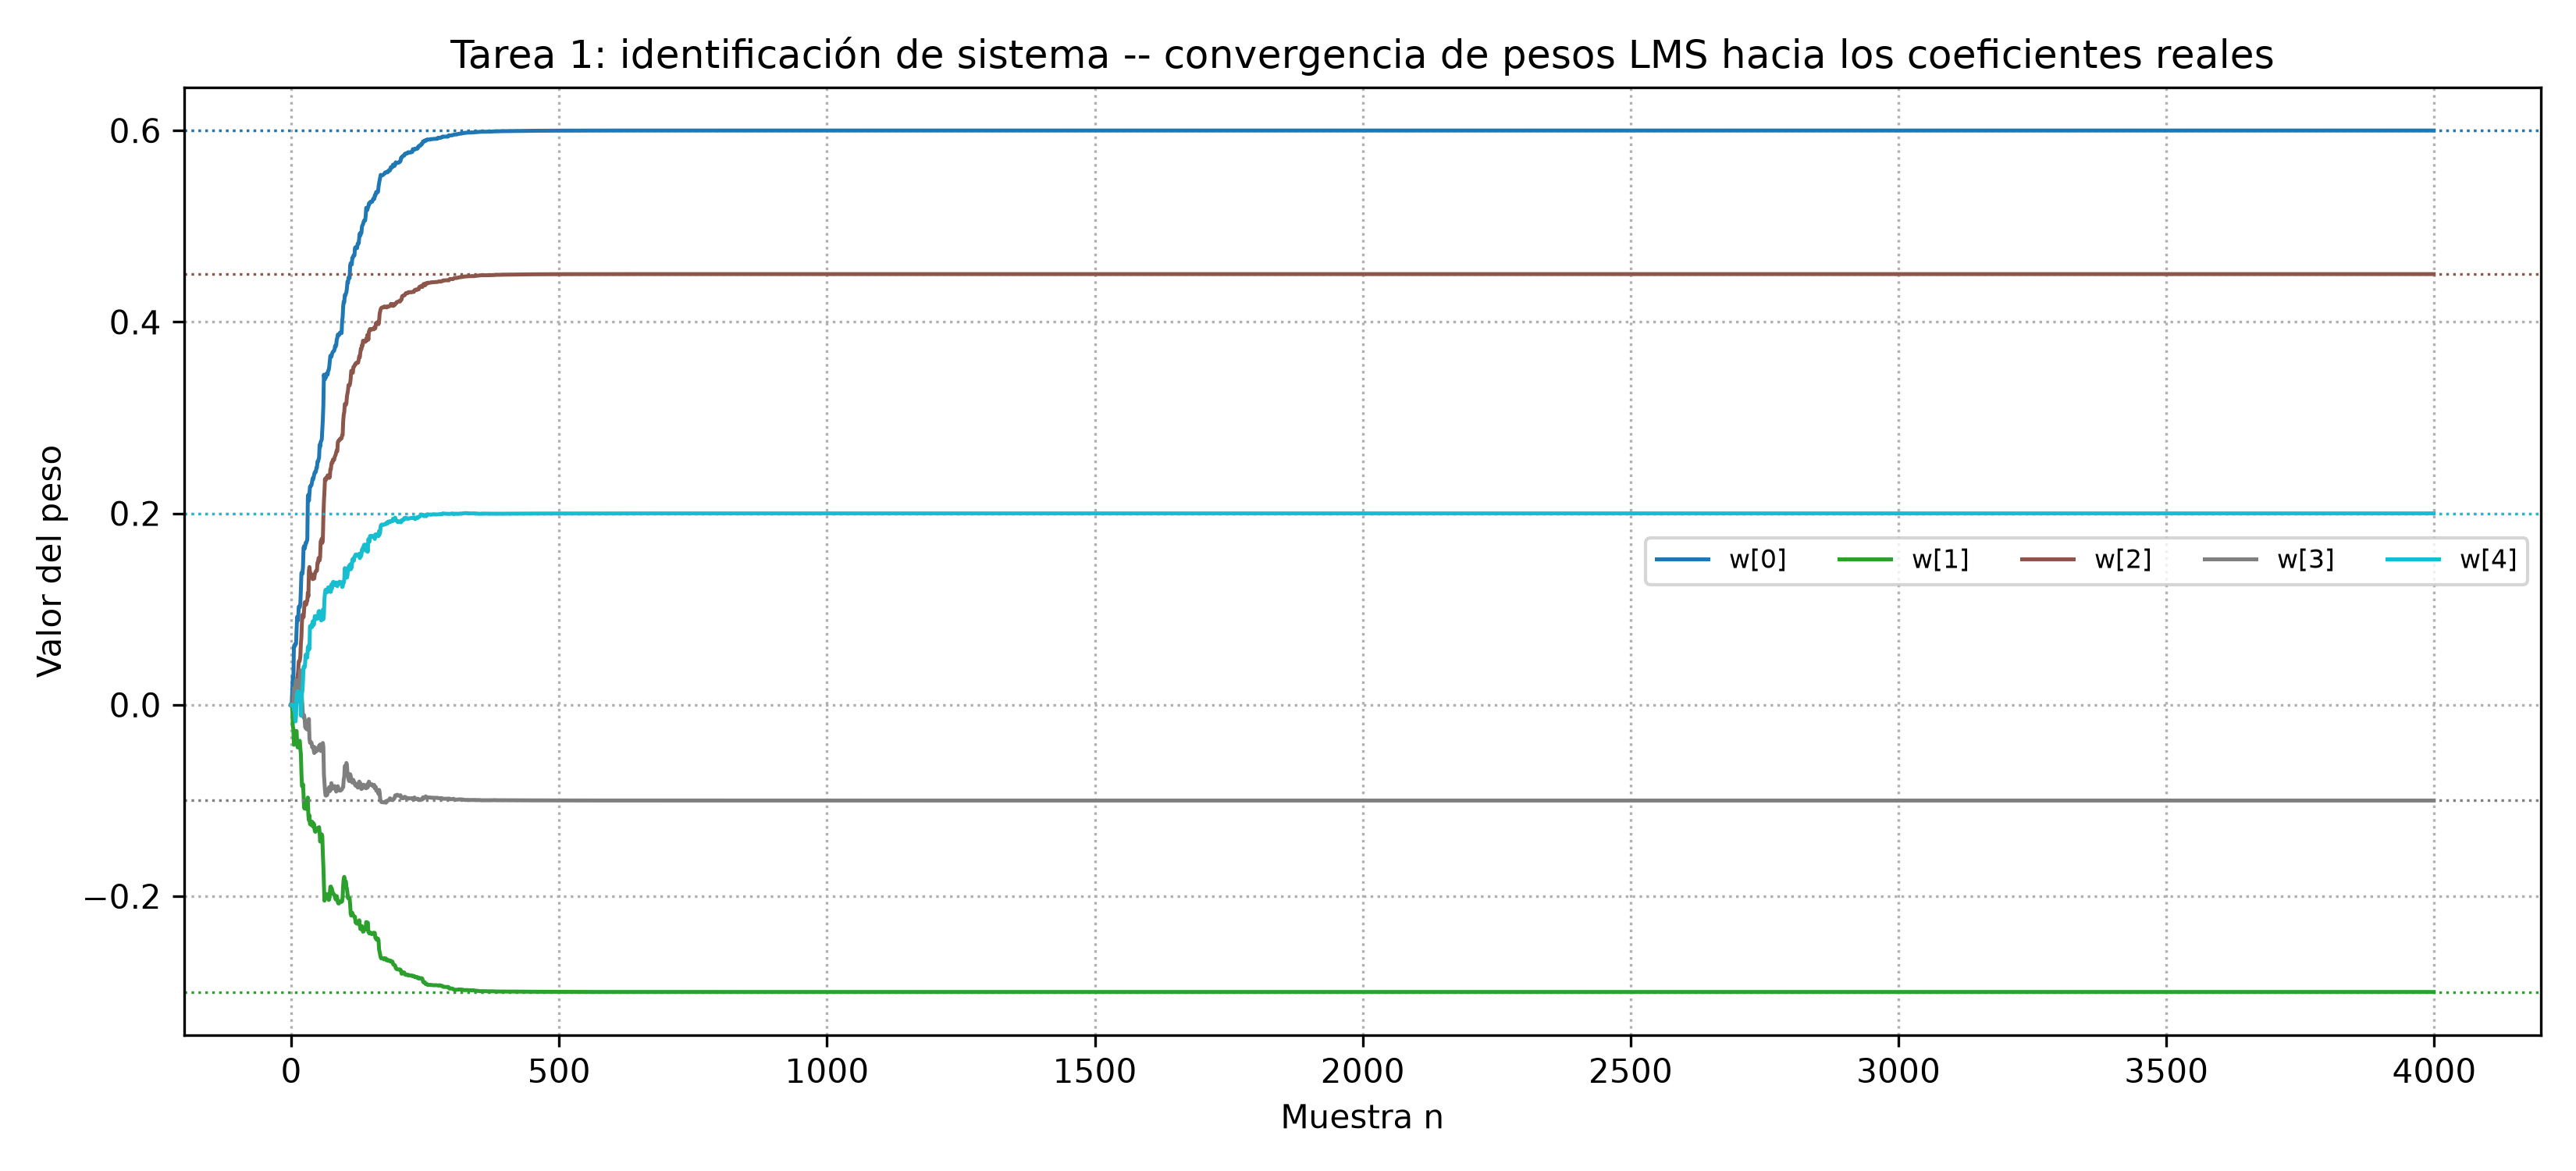
\includegraphics[width=\columnwidth]{work_eleven_t1_weight_convergence.png}
\caption{LMS: convergencia de los 5 pesos adaptados hacia los coeficientes reales del sistema FIR desconocido. Cada traza corresponde a un coeficiente individual, mostrando una convergencia monótona sin oscilación residual apreciable.}
\label{fig:work_eleven_t1_w}
\end{figure}

\begin{figure}[!t]
\centering
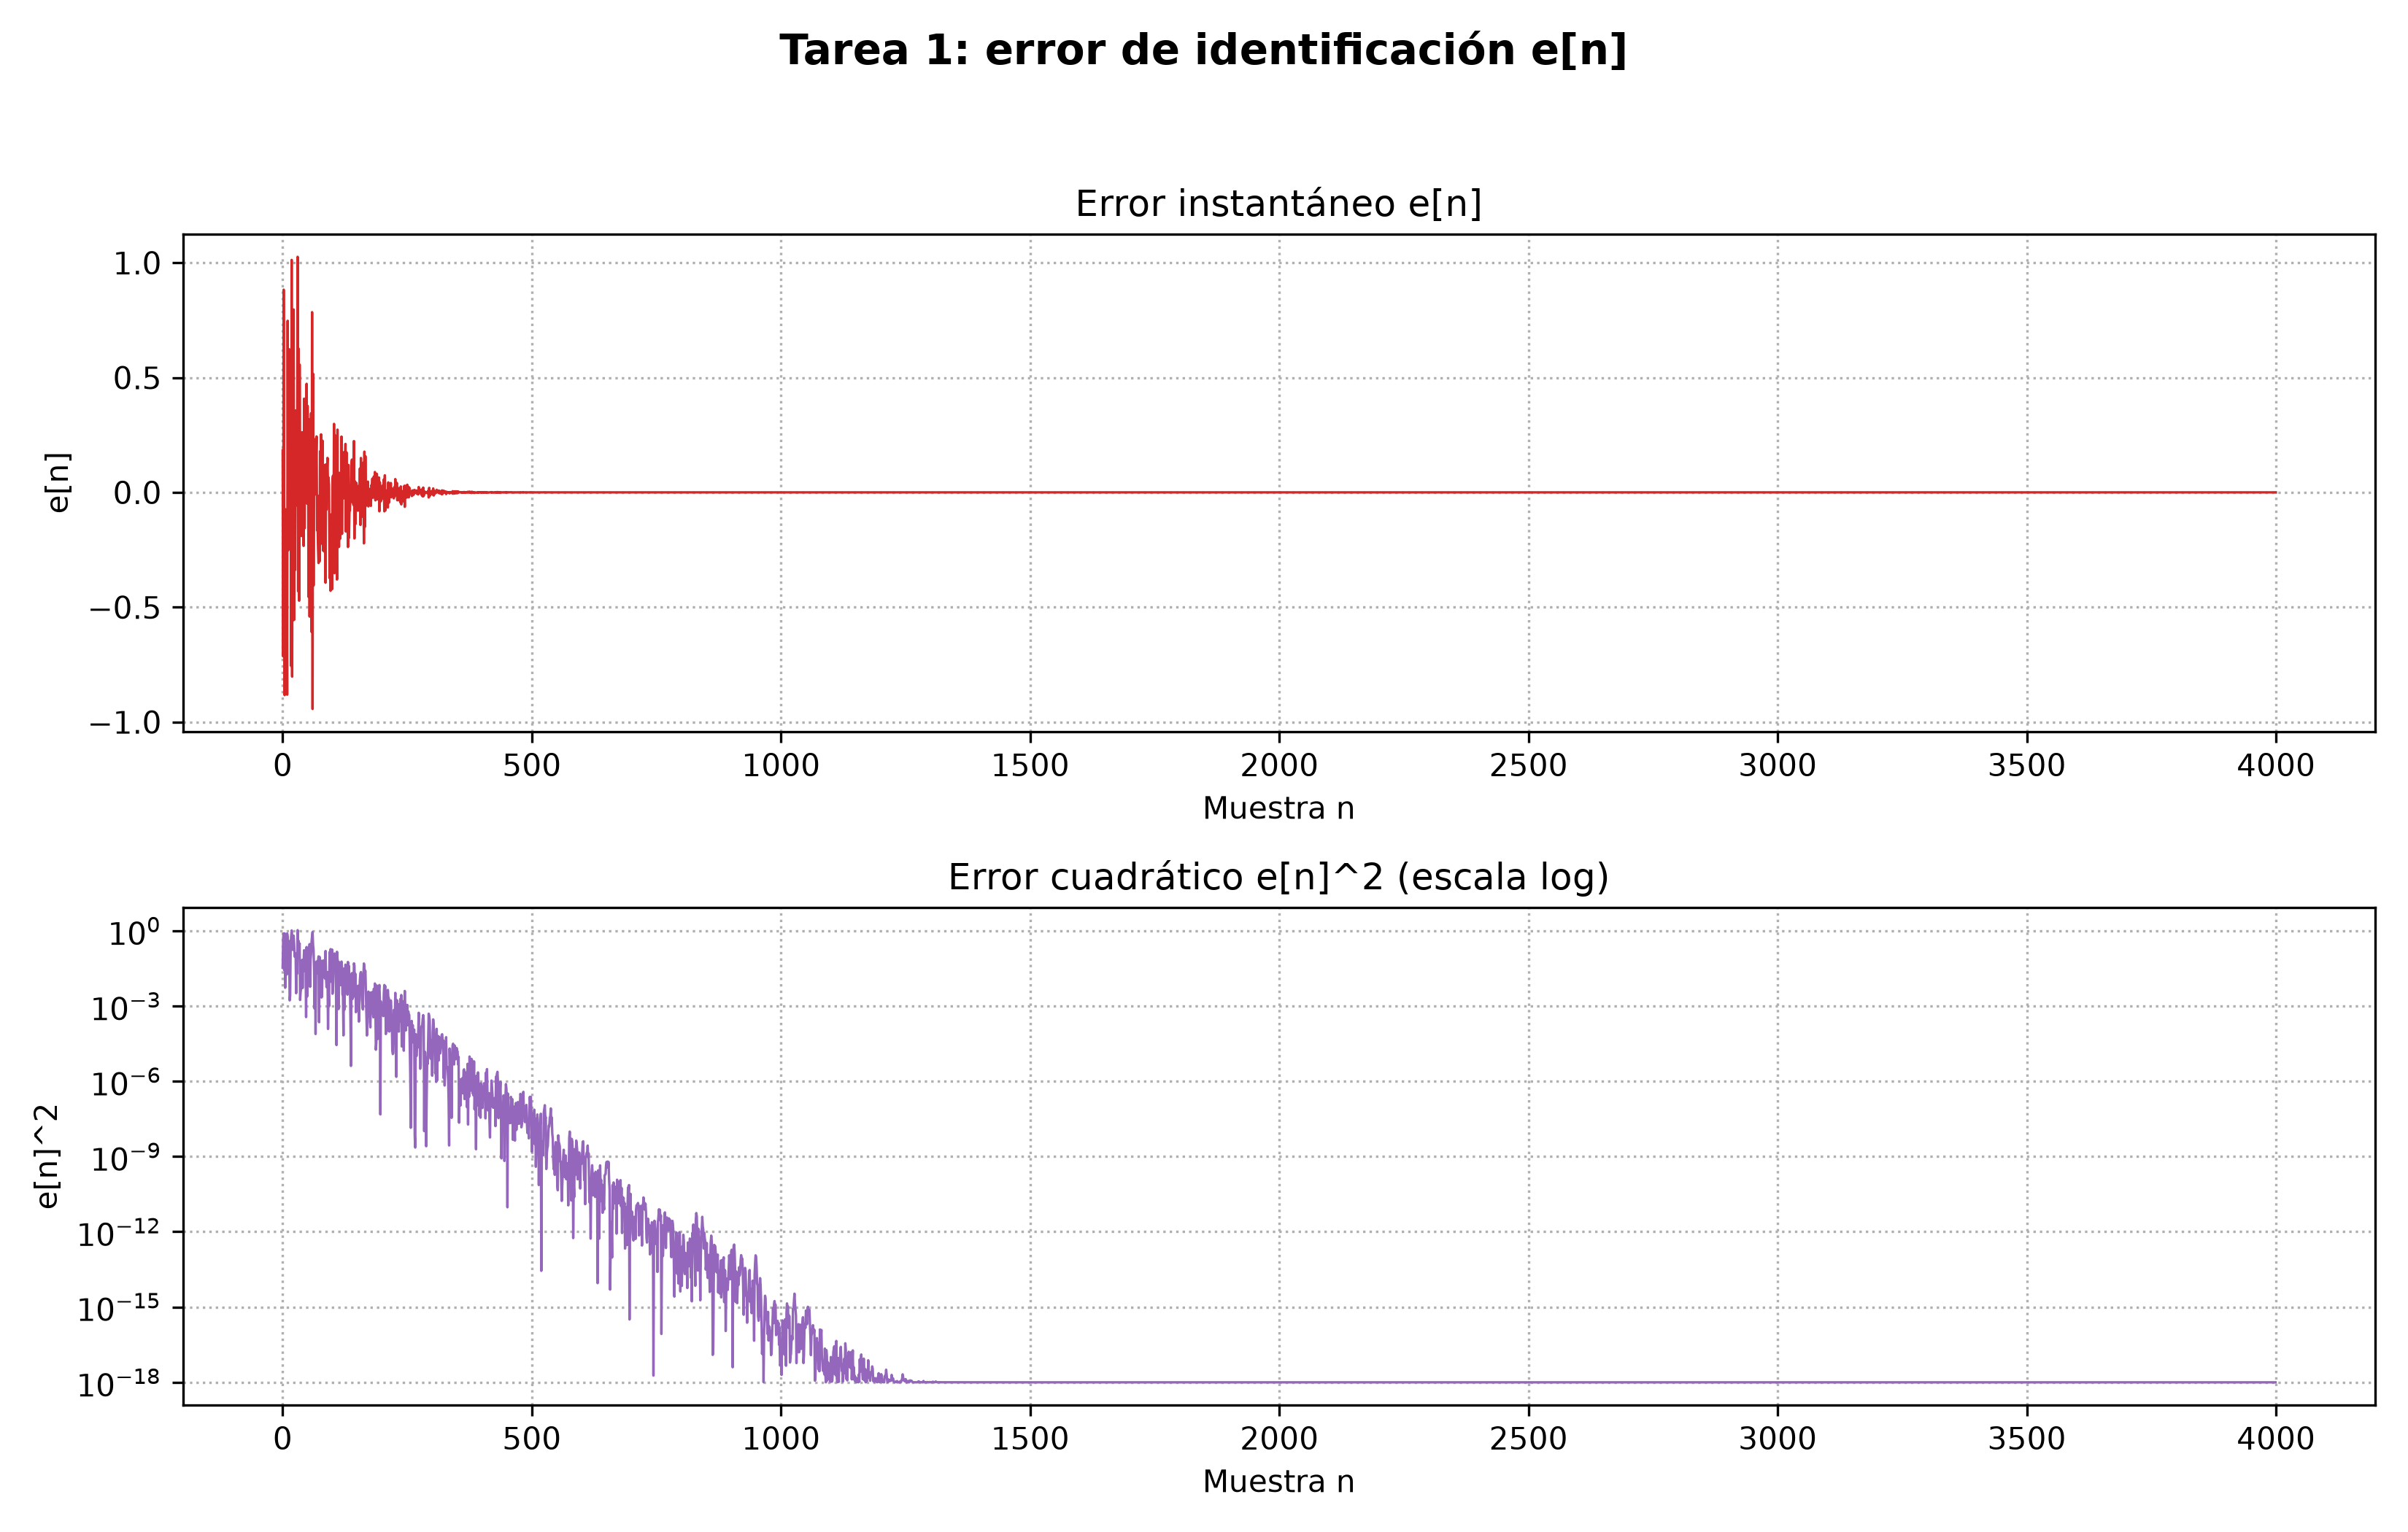
\includegraphics[width=\columnwidth]{work_eleven_t1_identification_error.png}
\caption{LMS: norma del error de identificación $\lVert w[n] - w_{\text{real}} \rVert$ en función de la iteración, en escala que evidencia el decaimiento exponencial característico del descenso de gradiente estocástico.}
\label{fig:work_eleven_t1_e}
\end{figure}

\subsubsection{Cancelación adaptativa de ruido}

El segundo experimento implementa un esquema clásico de cancelación
adaptativa de ruido (\textit{Adaptive Noise Cancellation}, ANC) de dos
entradas: una señal primaria, que contiene la señal de interés
contaminada por ruido, y una señal de referencia correlacionada con ese
ruido pero sin contenido de la señal de interés —la configuración
típica cuando se dispone de un sensor adicional capaz de captar
predominantemente la fuente de ruido. El filtro LMS usa la referencia
de ruido como entrada $x[n]$ y la señal primaria contaminada como señal
deseada $d[n]$; a medida que converge, la salida del filtro $y[n]$ se
aproxima a la componente de ruido presente en la señal primaria, de
modo que el error $e[n] = d[n] - y[n]$ —que es la salida real de
interés del sistema, no un subproducto a minimizar— tiende hacia la
señal limpia original.

Se aplicó este esquema sobre dos señales de naturaleza distinta para
evaluar su robustez: un tono sintético de 60~Hz, elegido por
consistencia con el resto de esta serie de trabajos, y una grabación de
audio real (el mismo archivo \texttt{gato.ogg} usado en trabajos
anteriores de este repositorio, copiado localmente para mantener esta
carpeta autocontenida). En el caso del tono, la desviación estándar del
residuo —la medida de cuánto ruido queda tras el filtrado— cayó de
0.617 antes del filtrado a 0.135 después, una reducción de ruido de
aproximadamente 4.6 veces en términos de desviación estándar (y por lo
tanto, de más de 20 veces en potencia). El comportamiento sobre el
audio real (Fig.~\ref{fig:work_eleven_t2b}) confirma que el algoritmo
no depende de propiedades idealizadas de una señal sintética y
generaliza correctamente a una señal con contenido espectral más rico
y no estacionario.

\begin{figure}[!t]
\centering
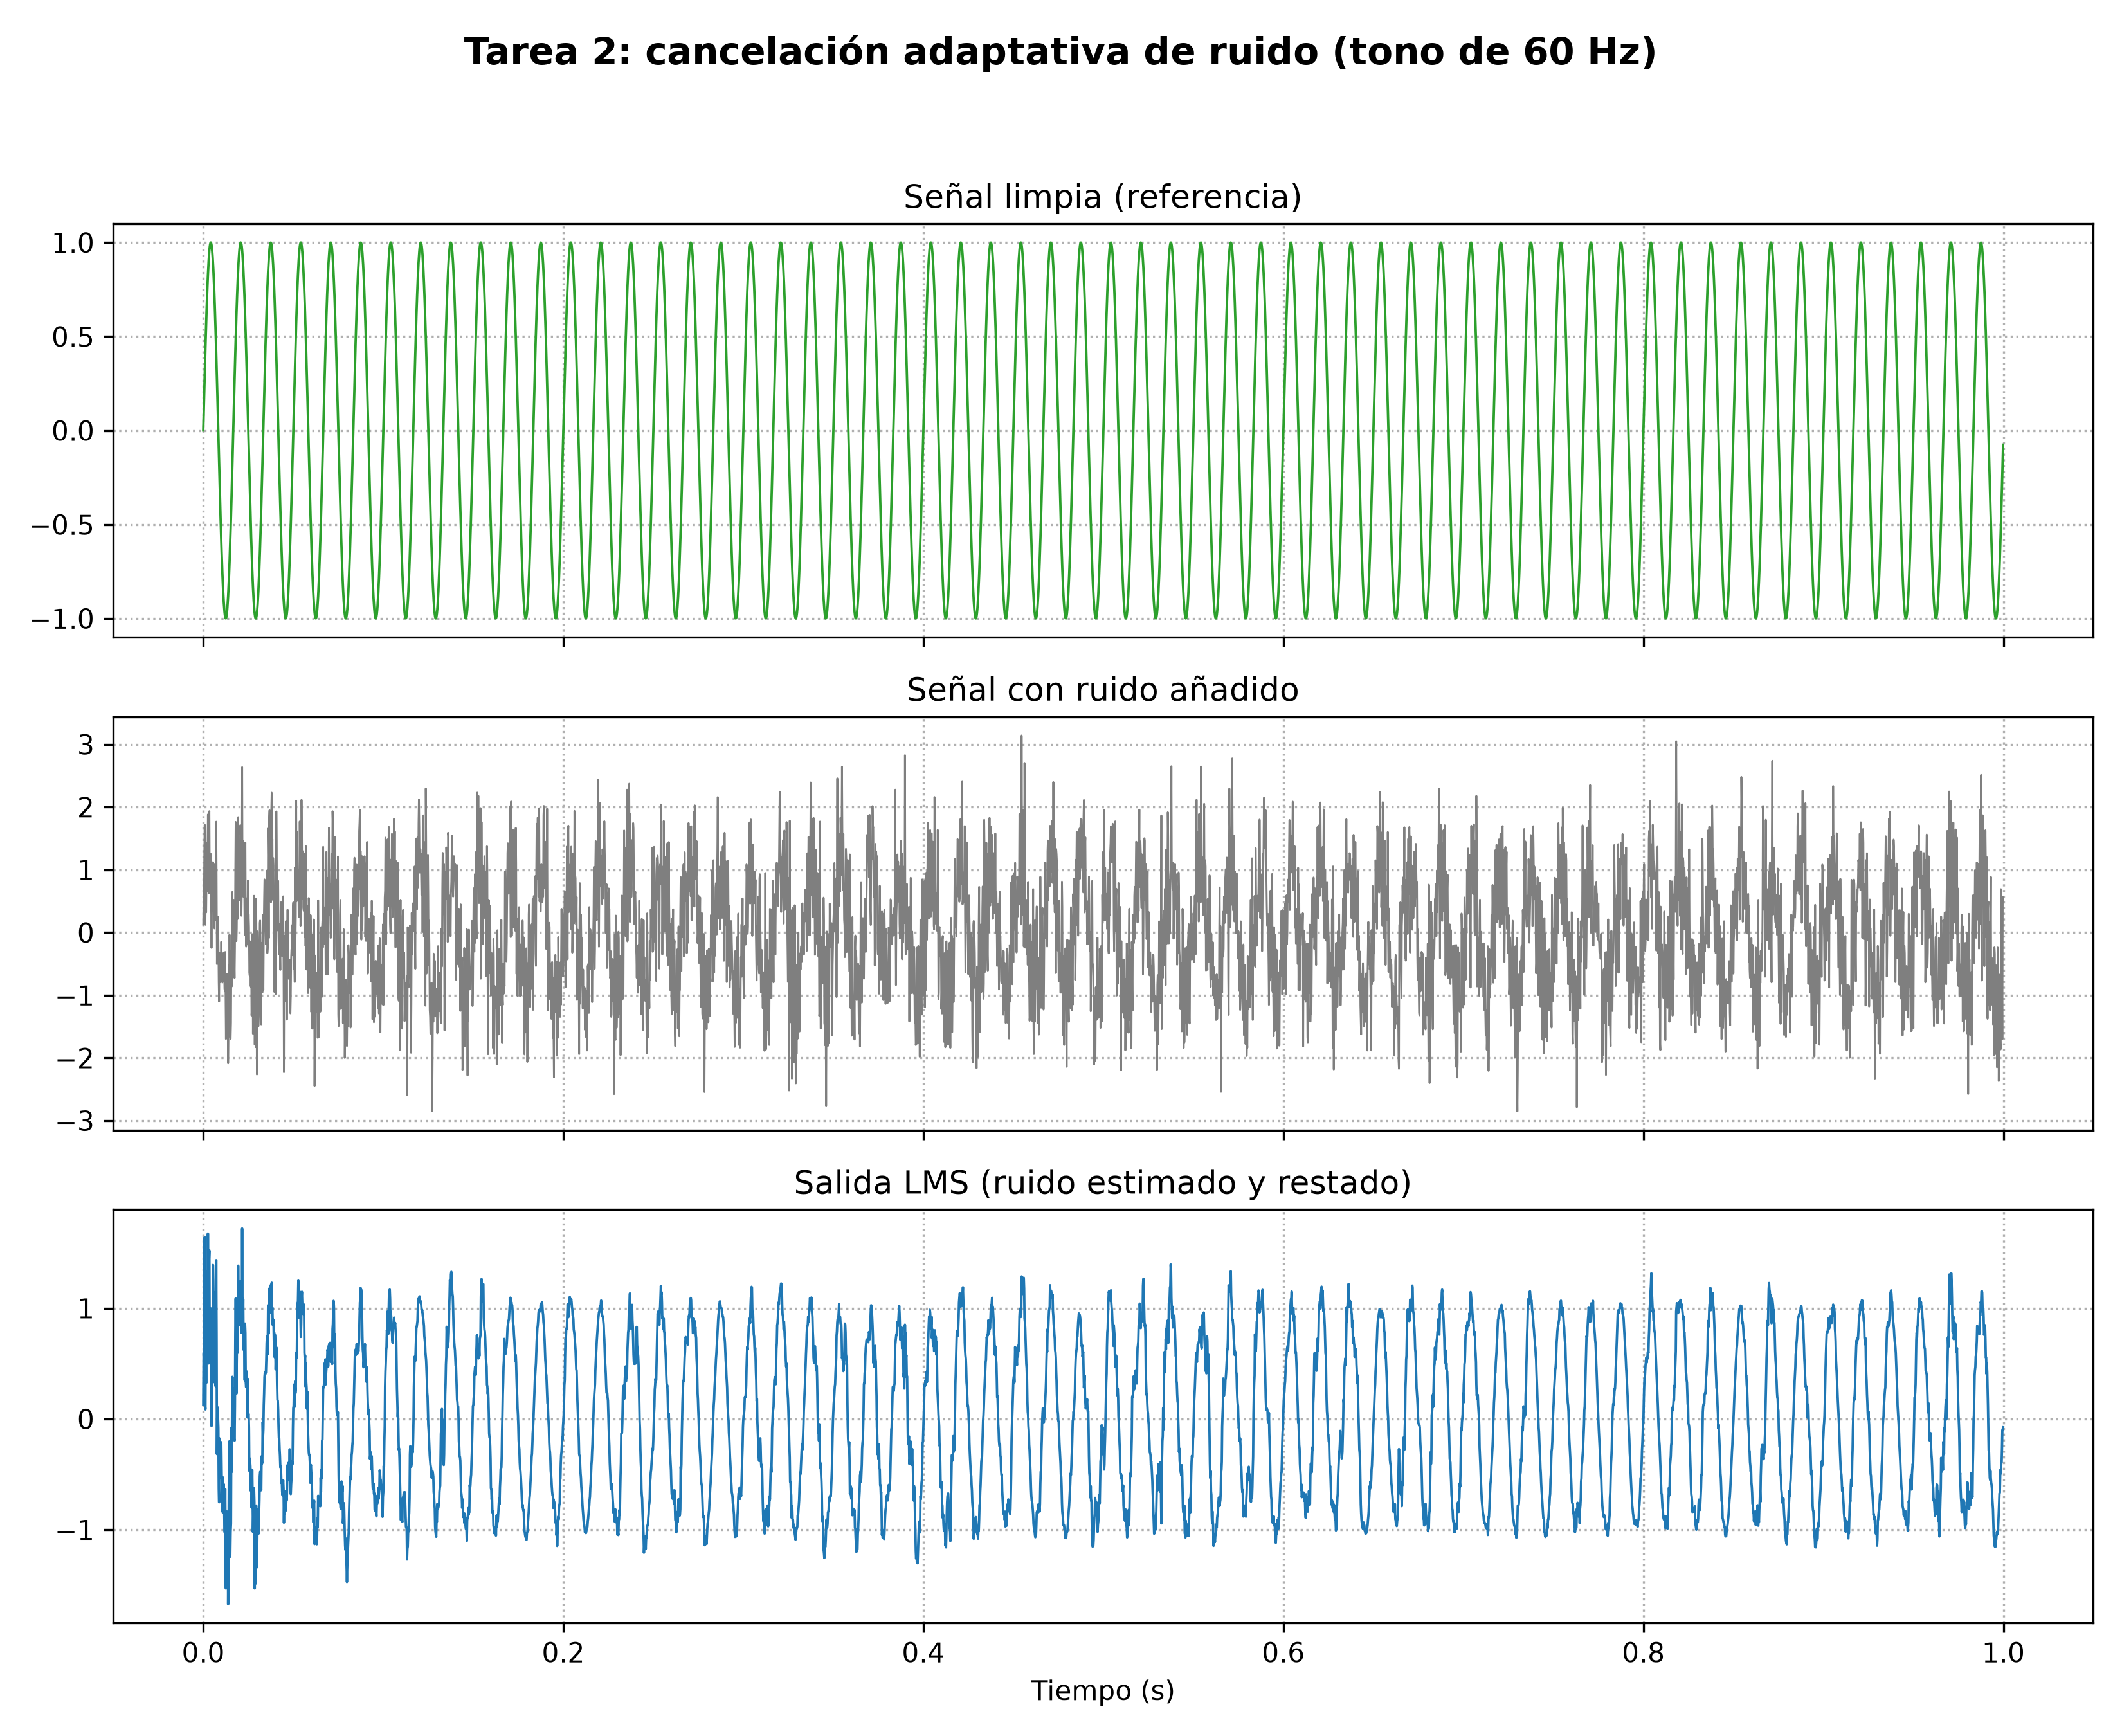
\includegraphics[width=\columnwidth]{work_eleven_t2_noise_cancellation_tone.png}
\caption{LMS: cancelación adaptativa de ruido sobre un tono de 60~Hz. De arriba a abajo: señal limpia de referencia, señal primaria contaminada, señal recuperada tras la cancelación.}
\label{fig:work_eleven_t2}
\end{figure}

\begin{figure}[!t]
\centering
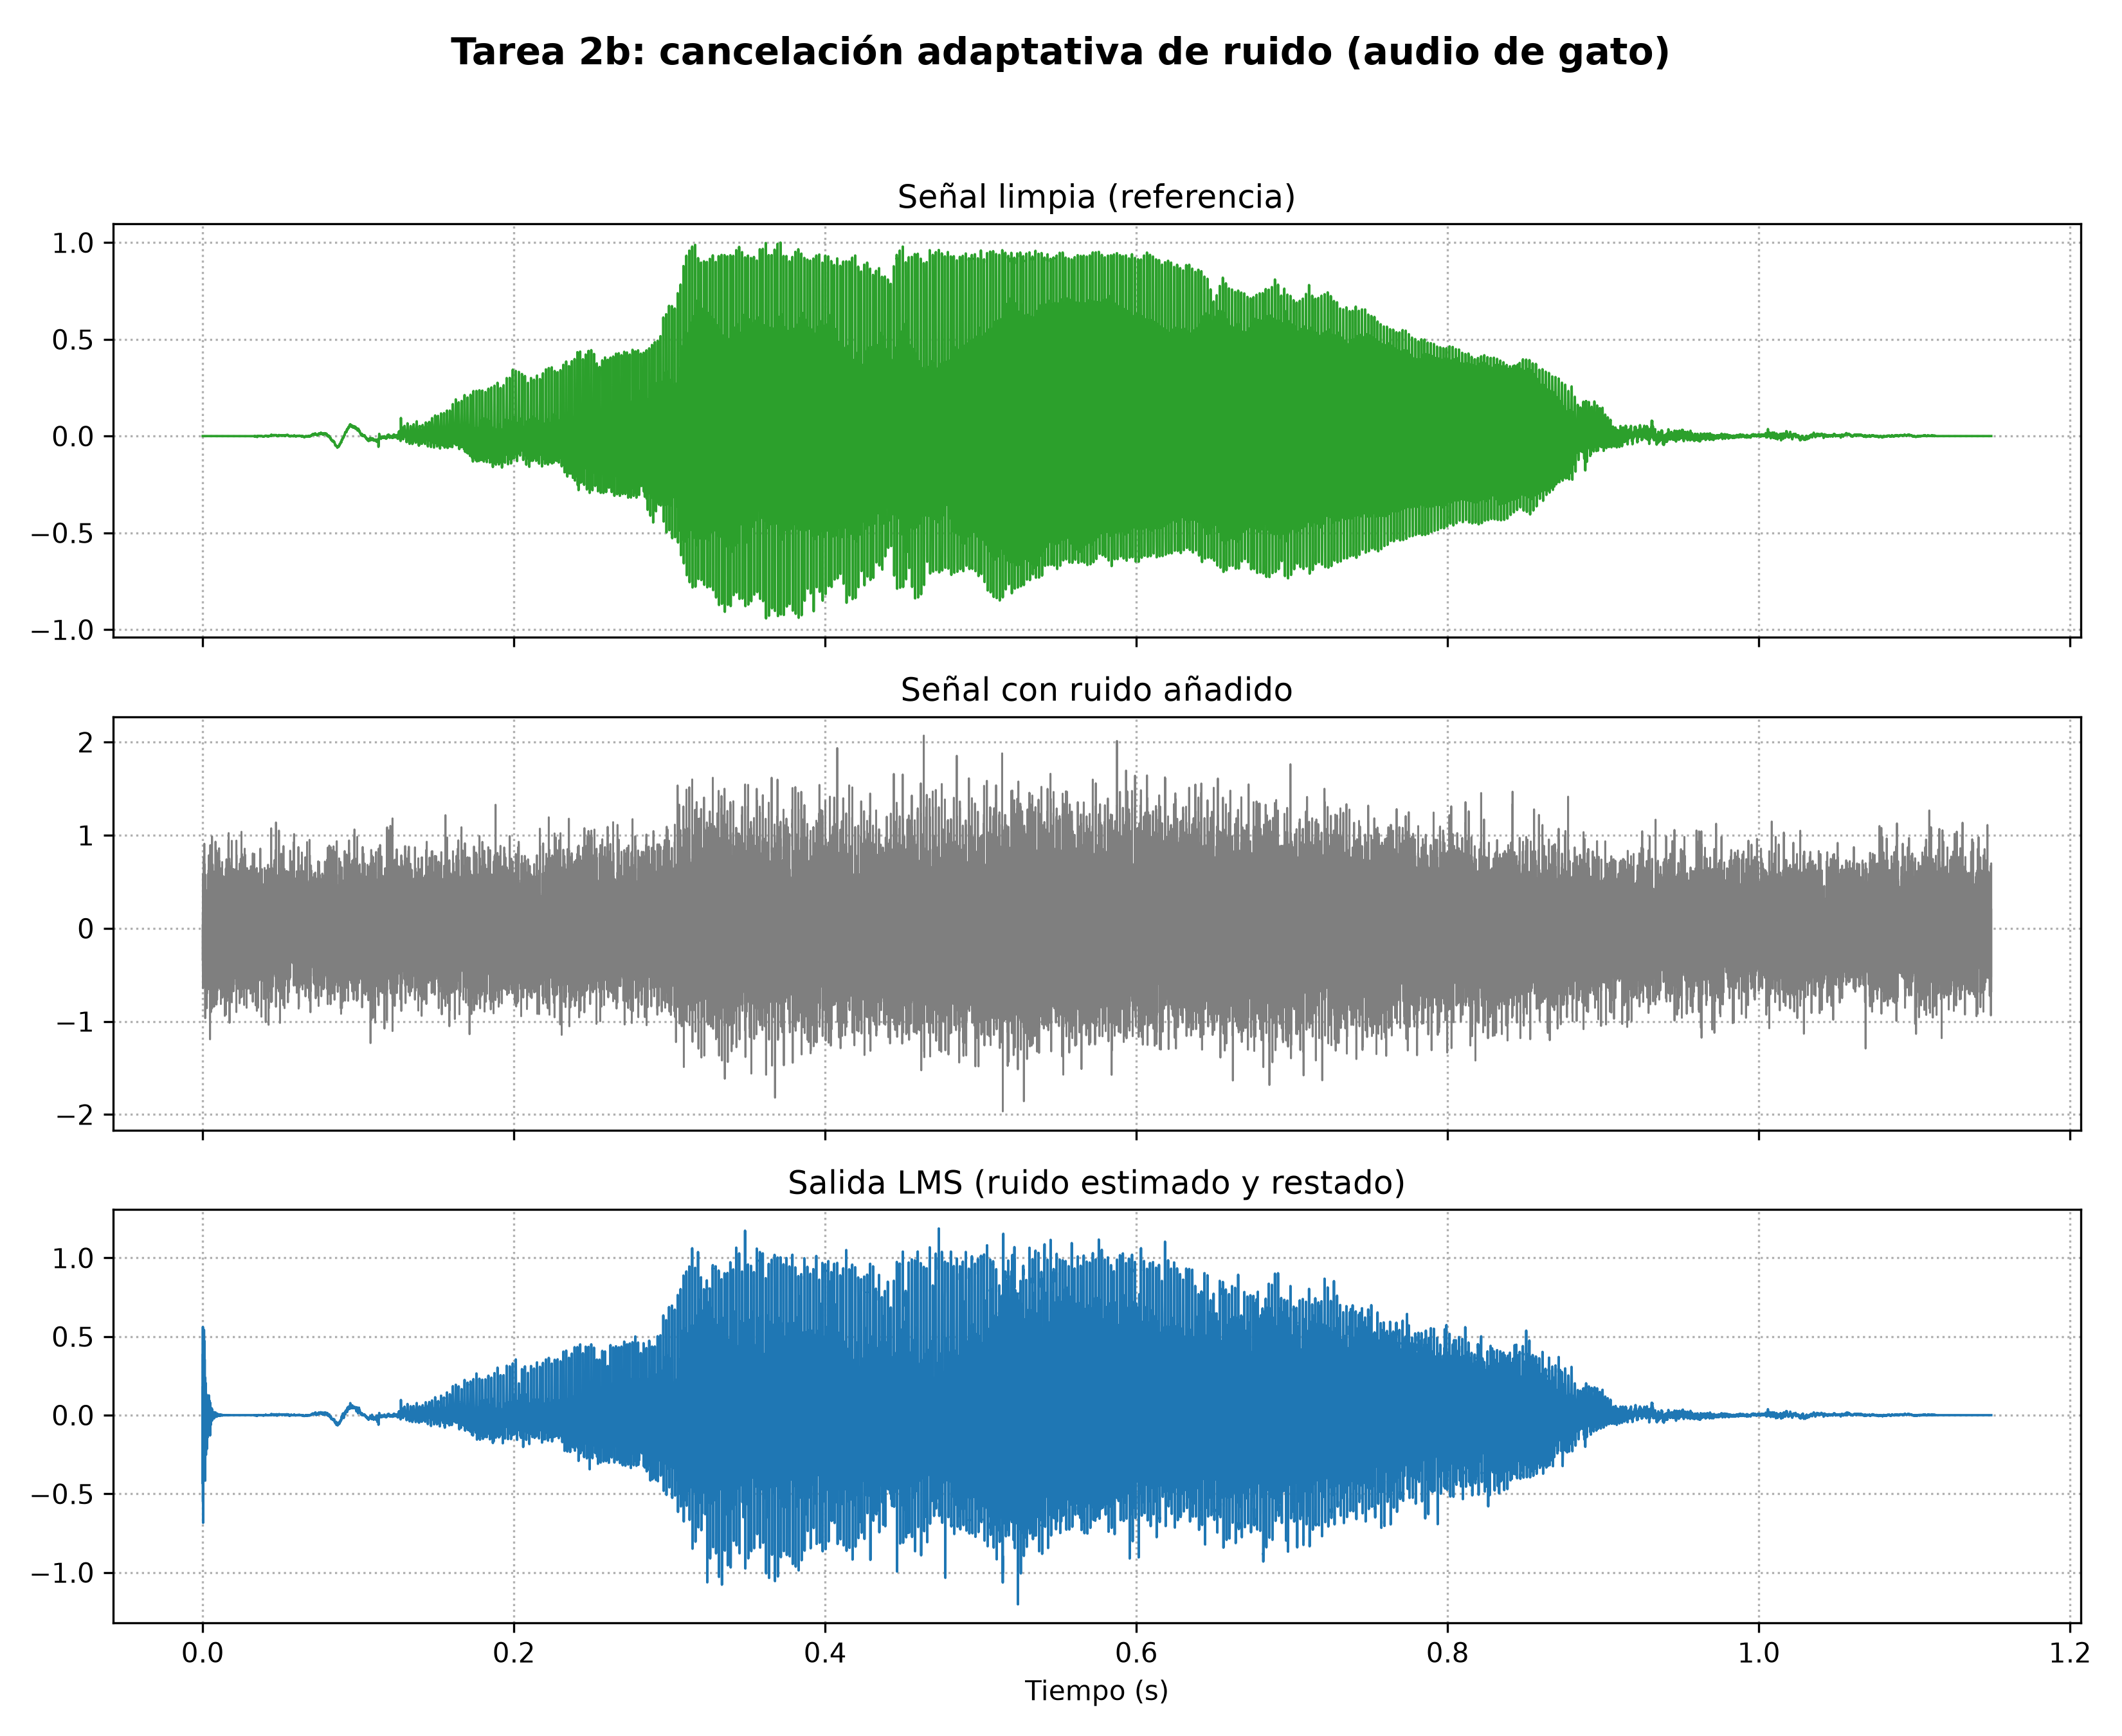
\includegraphics[width=\columnwidth]{work_eleven_t2b_noise_cancellation_cat.png}
\caption{LMS: cancelación adaptativa de ruido sobre una grabación de audio real, mostrando que el esquema de dos entradas generaliza más allá de señales sintéticas de banda angosta.}
\label{fig:work_eleven_t2b}
\end{figure}

\subsubsection{Convergencia frente al tamaño de paso $\mu$}

El tercer experimento caracteriza de forma sistemática el compromiso
velocidad/estabilidad discutido en la introducción, barriendo el mismo
problema de identificación de sistema sobre un conjunto de valores de
$\mu$ que abarca varios órdenes de magnitud
(Fig.~\ref{fig:work_eleven_t3}). Con $\mu = 0.001$, la convergencia es
notablemente lenta y, dentro del número de iteraciones ejecutado, queda
un error residual medible: el filtro todavía está en camino hacia la
solución óptima, no la ha alcanzado. Con $\mu$ en el rango de 0.01 a
0.1, la convergencia es rápida y el filtro alcanza un error
prácticamente nulo (limitado únicamente por la precisión numérica de
punto flotante), sin señales de oscilación o inestabilidad. Con
$\mu = 0.5$, en cambio, el filtro diverge de forma manifiesta,
acumulando error hasta desbordar numéricamente (de ahí la advertencia
de \textit{overflow} de NumPy registrada intencionalmente durante la
ejecución de pruebas, que documenta precisamente este comportamiento
esperado).

Este resultado experimental se corresponde de forma precisa con la
cota teórica de estabilidad de LMS, que establece que el algoritmo
converge en media cuadrática si y solo si
\begin{equation}
0 < \mu < \frac{2}{\lambda_{\max}},
\end{equation}
donde $\lambda_{\max}$ es el mayor autovalor de la matriz de
autocorrelación $R = E[x[n]\,x[n]^\top]$ de la entrada. Para una
entrada de ruido blanco con $N$ coeficientes y varianza $\sigma_x^2$,
la matriz de autocorrelación es aproximadamente $\sigma_x^2 I$, de modo
que todos sus autovalores son iguales a $\sigma_x^2$ y la cota se
simplifica a $\mu < 2/(N\sigma_x^2)$. Para la configuración usada en
este laboratorio ($N=5$ coeficientes, $\sigma_x^2 \approx 1$), esta
cota resulta en $\mu \lesssim 0.4$, consistente con la estabilidad
observada en $\mu \leq 0.1$ y la divergencia observada en $\mu = 0.5$,
que queda justo por encima del límite teórico.

\begin{figure}[!t]
\centering
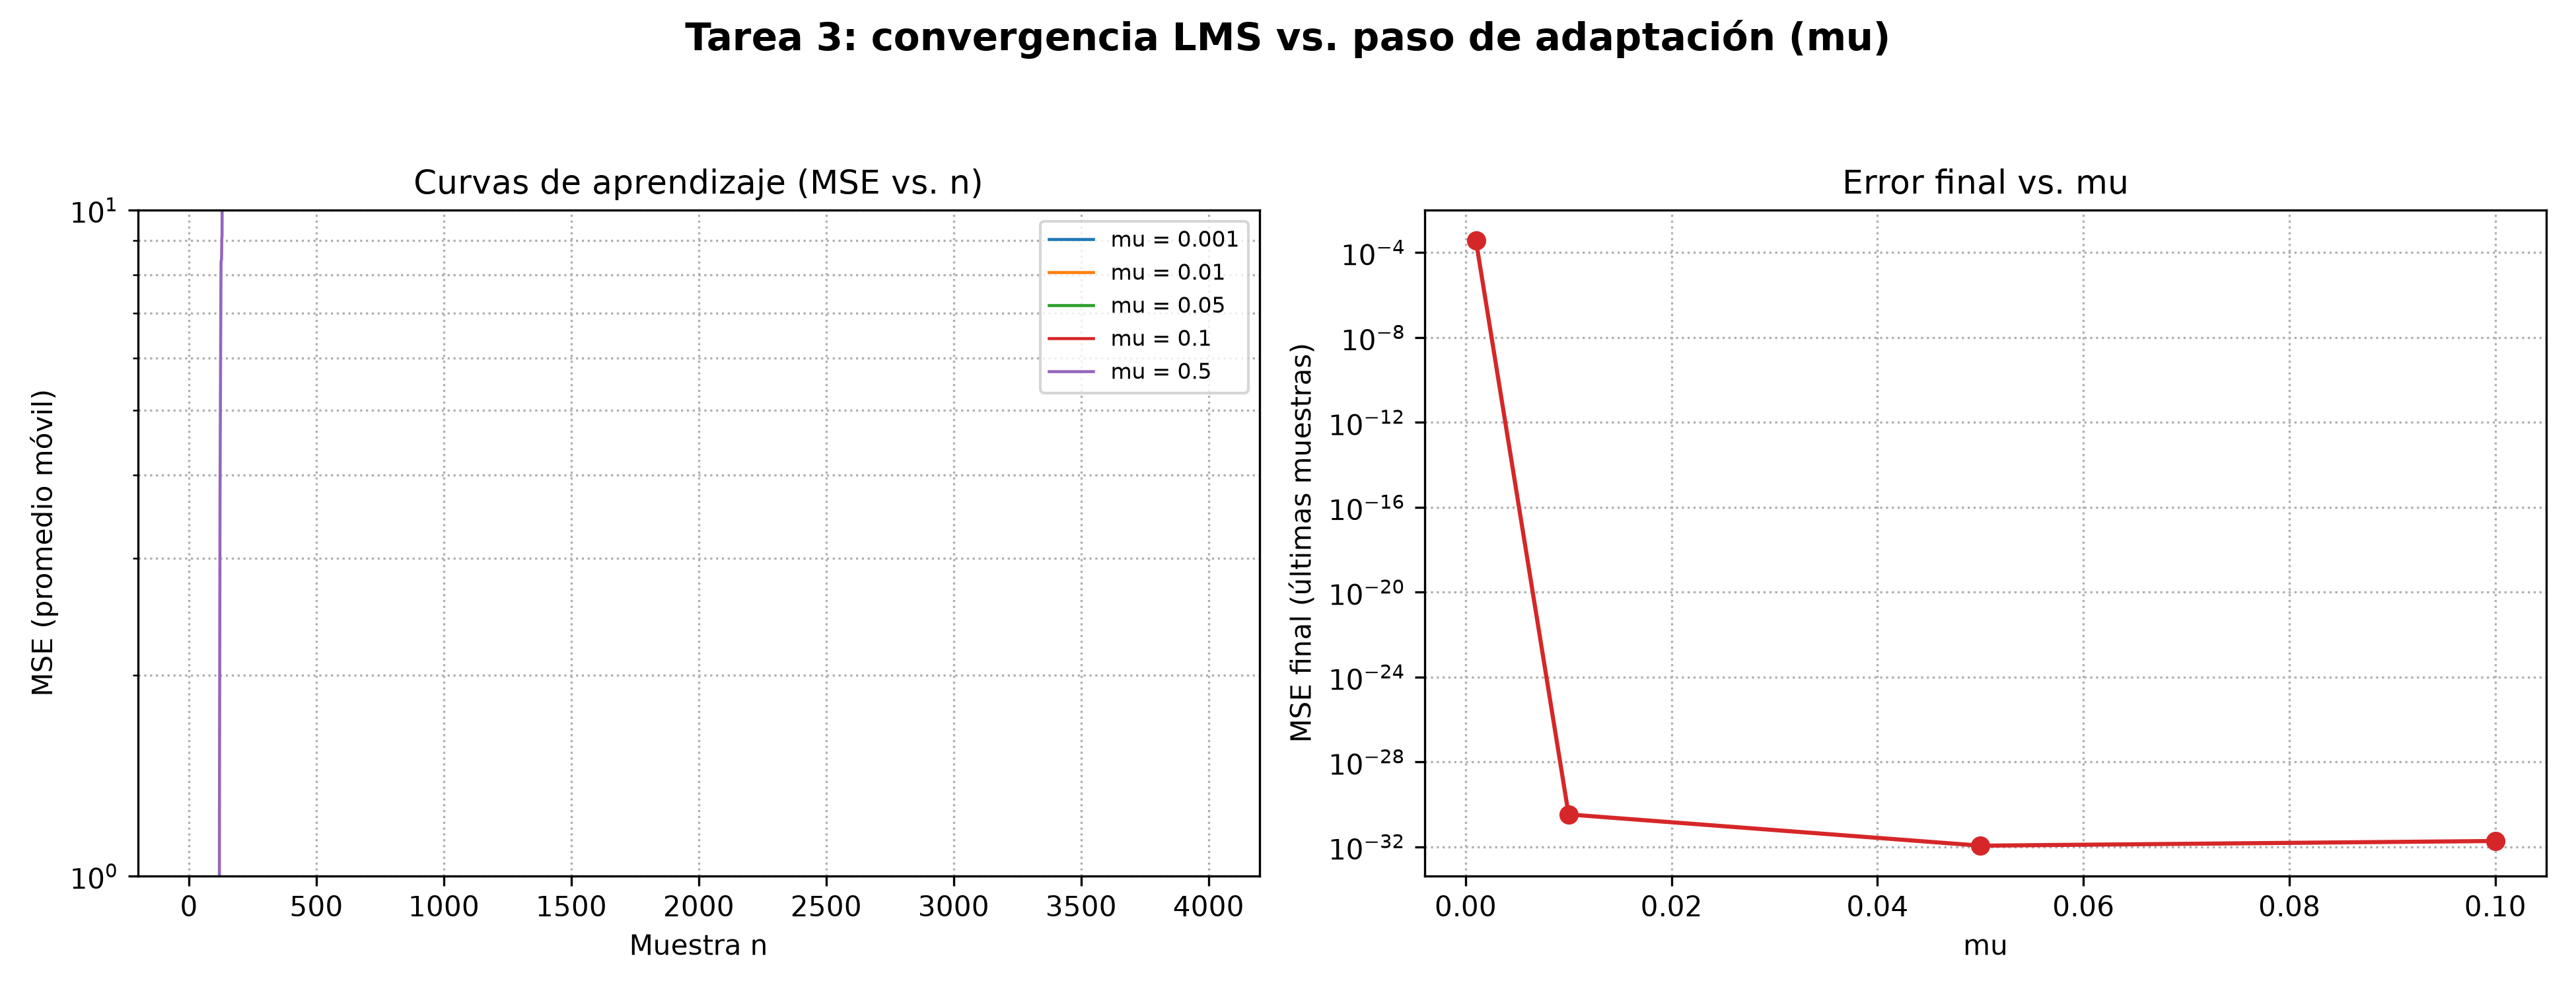
\includegraphics[width=\columnwidth]{work_eleven_t3_mu_sweep.png}
\caption{LMS: error cuadrático medio en estado estacionario en función de $\mu$ (escala logarítmica), evidenciando las tres regiones de comportamiento: convergencia lenta ($\mu$ pequeño), convergencia rápida y estable (región intermedia), y divergencia ($\mu$ por encima de la cota teórica $2/\lambda_{\max}$).}
\label{fig:work_eleven_t3}
\end{figure}
